%%%%%%%%%%%%%%%%%%%%%%%%%%%%%%%%%%%%%%%%%%%%%%%%%%%%%%%%%%%%%%%%%%%%%%%%%%%%
%%% Template para relat rio, trabalho, manual, tcc dissertacao ou tese
%%% Release 18/07/2013
%%%	Por Will D. Fonseca
%%% willdfonseca@yahoo.com.br
%%%%%%%%%%%%%%%%%%%%%%%%%%%%%%%%%%%%%%%%%%%%%%%%%%%%%%%%%%%%%%%%%%%%%%%%%%%%

%%%%%%%%%%%%%%%%%%%%%%%%%%%%%%%%%%%%%%%%%%%%%%%%%%%%%%%%%%%%%%%%%%%%%%%%%%%%%%%%%%%%%%%%%%%%%%%%%%%%%%%%%%%%%%%%%%%%
%%%%%%%%%%%%%%%%%%%%%%%%%%%%%%%%%%%%%%%%%%%%%%%%%%%%%%%%%%%%%%%%%%%%%%%%%%%%%%%%%%%%%%%%%%%%%%%%%%%%%%%%%%%%%%%%%%%%
%%%======================= Classe
%%% N o mexer neste parte %%%%%%%
%\documentclass[a4paper,12pt]{article}
%\documentclass[a4paper,12pt,twoside]{report}
\documentclass[a4paper,12pt,twoside]{scrreprt}

%\documentclass[a4paper,12pt]{scrreprt} 
% Aqui classe especifica o tipo de documento a ser criado.
% Gerar o documento como um report com a fonte base de onze pontos,usando papel A4.
% {report} Para relat rios maiores contendo diversos cap tulos, pequenos livros, teses de doutorado,...
% [twoside] paginas impares e pares

%%%%%%%%%%%%%%%%%%%%%%%%%%%%%%%%%%%%%%%%%%%%%%%%%%%%%%%%%%
%TC:ignore % For counting words
%%%%%%%%%%%%%%%%%%%%%%%%%%%%%%%%%%%%%%%%%%%%%%%%%%%%%%%%%%

\usepackage{scrhack}
% Ative caso use ``scrreprt'', este pacote evita conlfito com o hyperref
\usepackage{url}
\usepackage{afterpage}
% Evita os erros de overfull
\hbadness=10000
\hfuzz=50pt

% Ajustando magerns para padrao % for easy management of document margins
\usepackage[a4paper,left=2.5cm,right=2.0cm,top=2.8cm,bottom=2.4cm]{geometry}

\usepackage{chngpage} % to easily change the margins of pages.
											% Caso precise folhas com margens especiais

%%%%%%%%%%%%%%%%%%%%%%%%%%%%%%%%%%%%%%%%%%%%%%%%%%%%%%%%%%
%%%======================= Entrada e Fontes
%\usepackage[ansinew]{inputenc} % please do not change!
 %Para configurar a codifica  o do arquivo de entrada (ex.: \usepackage[latin1]{inputenc} permite usar os caracteres acentuadas).
\usepackage[utf8]{inputenc}

\usepackage[brazilian]{babel} % The multilingual package. 
% O pacote babel especifica a linguagem/dialeto utilizada. O  ltimo torna-se o padr o
% Ele acerta a hifenizacao e titulo/nome que ele coloca automaticamente.

\usepackage{setspace}

\usepackage[T1]{fontenc} 
\usepackage{ae} % Fonte virtual para arquivo PDF com fonte CMR codificado como T1 (este pacote resolve problemas do mapeamento de fontes acentuadas do Computer Modern no documento PDF).

% Font encoding package. Especifica qual codifica  o de fontes o Latex deve usar.
% 1.OT1 eh a codificacao de 7-bits: Ingl s, alem o, latin, etc.
% 2.T1 eh a codificacao de 8 bits (Cork encoding): mais ligaduras.
%    Apropriado para documentos com caracteres acentuadas como portugues,
%    o que habilita a usar algumas "ligaduras" adicionais e regra de 
%    hifeniza  o das palavras acentuadas
% A especifica  o da regra de hifeniza  o na lista \hyphen{}, 
% das caracteres acentuadas requer codificacao de 8 bits 
% (T1 como opcao do fontenc).
% Quando gera PDF, tamb m pode precisar da codifica  o de 8 bits para letras acentuadas ou s mblos adicionais.

%%% Permit fonts at arbitrary sizes. %See for detail http://www.tex.ac.uk/cgi-bin/texfaq2html?label=fontunavail
\usepackage{type1cm}
%\usepackage{type1ec}
\usepackage{fix-cm}           % Permit Computer Modern fonts at arbitrary sizes.
\usepackage{fourier-orns}
\usepackage{lmodern}

%%%%%%%%%%%%%%%%%%%%%%%%%%%%%%%%%%%%%%%%%%%%%%%%%%%%%%%%%%
%%%======================= Espaco adicional no listofigures
\makeatletter
\renewcommand*\l@figure{\@dottedtocline{1}{1.5em}{2.9em}}
\makeatother
%The length 1.5em is the space from the left margin to every line in the list of figures, whereas 2.3em is the space reserved for the number of every figure. 
%It seems that you need to increase this length. Put in the preamble of your document something like:
%%%%%%%%%%%%%%%%%%%%%%%%%%%%%%%%%%%%%%%%%%%%%%%%%%%%%%%%%%
%%%======================= Matematica
\usepackage{amsmath, amssymb, amsfonts}
% amsmath carrega diversos pacotes do AMS para incrementar o ambiente matematico.
% Os pacotes amssymb e amsmath sao mais usados
% amssymb Carrega diversos simbolos matematicos adicionais. 
% Este pacote carrega automaticamente o amsfonts 

\usepackage{amsthm}
%The amsthm package provides an enhanced version of LATEX's \newtheorem command
%for defining theorem-like environments.

\usepackage{array}
\usepackage{subeqnarray}
% Como visto anteriormente,cada equa  o recebe uma diferente refer ncia.Por m,se o
% usu rio desejar usar a mesma refer ncia para todas as equa  es   s  utilizar o pacote chamado
% subeqnarray. That the individual lines are numbered like 1a, 1b, 1c, etc.
% Isto  : coloca numeracao 3.7a , 3.7b , etc ....nas equacoes, usar \slabel (ex: \slabel{sub2}a&=&b-5)

\usepackage{chemarrow} %Seta em cima da seta

\usepackage{mathrsfs}
% Support use of the Raph Smith's Formal Script  font in mathematics. Provides a \mathscr command, rather than overwriting the standard \mathcal command, as in calrsfs.

% More math fonts
\usepackage{upgreek}
\usepackage{dsfont} 
%\usepackage{latexsym}
%%%%%%%%%%%%%%%%%%%%%%%%%%%%%%%%%%%%%%%%%%%%%%%%%%%%%%%%%%
%%%======================= Tabelas 
\usepackage{array,tabularx}
% array, Arrays e tables (tabular) com colunas formatados

% tabularx, Tabulars that widen automatically. 
% Paraigualar colunas desejadas do array/table, mantendo o c lculo automatico para largura.
%%%%%%%%%%%%%%%%%%%%%%%%%%%%%%%%%%%%%%%%%%%%%%%%%%%%%%%%%%
%%%======================= Imagens 
\usepackage{graphicx,wrapfig}
% Pacote padr o para incluir figuras, usando comando \includegraphics[]{}. O nome do drive pode ser indicado na % op  o do pacote. Ex.: \usepackage[dvips]{graphicx).

% Figuras.pdf Se opacote graphicx for usado como opcional[pdftex]fica poss vel inserir
% figuras no formato *.pdf,neste caso o documento n o poder  ser compilado como latex e
% sim como pdfatex. Deve-se conferir se seu sistema oferece este recurso.
% Ex: \usepackage[pdftex]{graphicx}
% ver apostila_latex.pdf Figuras.jpg,.png,.pdf 

\usepackage{caption} %para fazer captionof
%\setlength{\captionmargin}{10pt}

\usepackage{rotating}  	% Package for rotating things
\usepackage{calc} 			% ? precisa para o newenvironment{onde}, junto com o amsmath
% calc, pacote para efetuar c lculo aritm tico,  til para calcular comprimento e valores de contadores.
% ex: altura de letra, comprimento de palavra
%\setcounter{x}{7/2}
%\setcounter{y}{3*\real{1.6}}
%\setcounter{z}{3*\real{1.7}}
%will assign the value 3 to the counter x, the value 4 to y, and the value 5 to z.
%This truncation also applies to intermediate results in the sequential computation
%of a composite expression; thus, the following command
%%%%%%%%%%%%%%%%%%%%%%%%%%%%%%%%%%%%%%%%%%%%%%%%%%%%%%%%%%
%%%======================= Texto
\usepackage{color}         											% para letras e caixas coloridas
\usepackage[usenames,dvipsnames]{xcolor}        % para letras e caixas coloridas possivel usar RGB, CMYK, etc

\usepackage{indentfirst} 												% Indenta a primeira linha do section/chapter

%\usepackage{multicol, wasysym, xspace, fancyhdr, shapepar}
\usepackage{multicol, wasysym, xspace, fancyhdr, shapepar, float}

\usepackage{subfig}
\DeclareSubrefFormat{myparens}{#1~(#2)}
\captionsetup[subfloat]{subrefformat=myparens,labelformat=parens,position=bottom,font={normalsize,rm}}

% - float, Improves the interface for defining floating objects such as figures and tables.
% - subfigure, Provides support for the manipulation and reference of small or  sub  figures and tables within  % a single figure or table environment. 
% - Multicol defines a multicols environment which typesets text in multiple columns (up to a maximum of 10), and %(by default) balances the end of each column at the end of the environment.
% - wasysym, The WASY2 (Waldi Symbol) font by Roland Waldi provides many glyphs like male and female symbols  
% and astronomical symbols, as well as the complete lasy font set and other odds and ends. 
% - xspace, controla o espa o de acordo com o que segue,  til para escrever macro.
% - fancyhdr, controle extensivo sobre cabe alho e rodap  da p gina. Cabe alho e rodapeh de forma sofisticada.
% - shapepar is a macro to typeset paragraphs in a specific shape. Molda o texto em uma certa forma.
% \; \, \: sao tipos de espa amento. \! eh um espa o negativo. \quad \qquad es amento positivo maior

%%%%%%%%%%%%%%%%%%%%%%%%%%%%%%%%%%%%%%%%%%%%%%%%%%%%%%%%%%
%%%======================= URL 
\usepackage{url}	% With the url package (\usepackage{url}) you can enter URLs like this: \url{http://www.stack.nl/~jwk/latex/}. 
\usepackage{multirow}
%Chamar PDF em pagina especifica \href{MasterF.pdf#page.32}{here}
%%%%%%%%%%%%%%%%%%%%%%%%%%%%%%%%%%%%%%%%%%%%%%%%%%%%%%%%%%
%%%======================= Latex
\usepackage{makeidx}
% para criar  ndice remissivo. Coloque o comando \makeindex no preamble e use \index{} para adicionar um  tem %no indice remissivo. O \printindex serve para colocar o  ndice remissivo no local desejado. Note que precisar  %a seguinte sequ ncia de execuss o: latex, makeindex, latex, latex para criar corretamente o  ndice remissivo %(caso use bibtex tamb m, a sequ ncia ser  algo como latex, makeindex, bibtex, latex, latex)
% gera indices em ordem alfabetica, 
\makeindex % fa a o makeindex

\usepackage{ifthen,xifthen}
% Provides commands of the form `if...then do... otherwise do...'. 
% ex: se a palavra tive um comprimento maior que X, fa a isso.
%%%%%%%%%%%%%%%%%%%%%%%%%%%%%%%%%%%%%%%%%%%%%%%%%%%%%%%%%%
%%%======================= Cabe alho
\def\shortauthor#1{\def\cabei{#1}}
\def\shorttitle#1{\def\cabeii{#1}}
% \def nao da conflito entre arquivos multiplos
% definicoes para rechamar informacoes. Neste caso, dados que irao aparecer no cabe alho.
\newcommand{\Index}[1]{#1\index{#1}} 
%%%%%%%%%%%%%%%%%%%%%%%%%%%%%%%%%%%%%%%%%%%%%%%%%%%%%%%%%%%%%%%%%%%%%%%%%%%%%%%%%%%%%%%%%%%%%%%%%%%%%%%%%%%%%%%%%%%%
%%% EDIT HERE PDF INFO %% Informar titulo, autores, ...
%%%%%%%%%%%%%%%%%%%%%%%%%%%%%%%%%%%%%%%%%%%%%%%%%%%%%%%%%%%%%%%%%%%%%%%%%%%%%%%%%%%%%%%%%%%%%%%%%%%%%%%%%%%%%%%%%%%%
\usepackage{datetime} % to get automaticallly the date

\title{Template para trabalhos.}

\author{William D. Fonseca}
\shorttitle{ \mbox{} }
\shortauthor{ \mbox{} }

\pdfinfo
{  /Author (William D. Fonseca)
   /Title  (NLR Report: Developmets with beamforming for a hard cylinder array.)
   /CreationDate (D:\pdfdate) %D:YYYYMMDDHHmmss
   /Subject (NLR, Beamforming, Acoustics, Cylinder, Array)
   /Keywords (NLR, Beamforming, Acoustics, Cylinder, Array)
}
%%%%%%%%%%%%%%%%%%%%%%%%%%%%%%%%%%%%%%%%%%%%%%%%%%%%%%%%%%%%%%%%%%%%%%%%%%%%%%%%%%%%%%%%%%%%%%%%%%%%%%%%%%%%%%%%%%%%
%%%%%%%%%%%%%%%%%%%%%%%%%%%%%%%%%%%%%%%%%%%%%%%%%%%%%%%%%%%%%%%%%%%%%%%%%%%%%%%%%%%%%%%%%%%%%%%%%%%%%%%%%%%%%%%%%%%%
%%%======================= Cite 
%\usepackage{citesort}
%The citesort package sorts the numbers and detects consecutive sequences, so creating  [2 4,6] .
\usepackage{notoccite}		%Counting the references from text not from list of figures, associated to the notoccite.sty file. at current directory
%%%%%%%%%%%%%%%%%%%%%%%%%%%%%%%%%%%%%%%%%%%%%%%%%%%%%%%%%%
%%%======================= N veis 
\addtocounter{secnumdepth}{1}	%%%% para 4 n veis enumerados
\addtocounter{tocdepth}{1}   	%%%% para fazer os 4 n veis aparecer no toc
%%%%%%%%%%%%%%%%%%%%%%%%%%%%%%%%%%%%%%%%%%%%%%%%%%%%%%%%%%
%%%======================= PDF functions 
\pdfminorversion=7     %Faz com que n o apare a a mensagem de warning sobre a vers o do pdf quando compilado.
\pdfimageresolution300
\pdfcompresslevel8	   %Nivel de compressao do PDF

\usepackage{pdfpages}	 %Incluir arquivos de PDF

\usepackage{lscape} 	 %Supplies a landscape environment, and anything inside is basically rotated. No actual page dimensions are changed. Using pdflscape instead of lscape when generating a PDF document will make the page appear right side up when viewed: the single page that is in landscape format will be rotated, while the rest will be left in portrait orientation.

%%% Links
\usepackage{ifpdf}
\ifpdf\usepackage{pdfpages}\fi
\usepackage[hyperindex,pagebackref=true]{hyperref}

%\hypersetup{bookmarks,colorlinks,breaklinks,plainpages=false,pdfpagelabels,linktocpage}
\hypersetup{plainpages=false,colorlinks,breaklinks,linktocpage,hypertexnames=true,naturalnames=false}
\hypersetup{linkcolor=red,citecolor=blue,filecolor=blue,urlcolor=blue} %Colorful
%\hypersetup{linkcolor=black,citecolor=black,filecolor=black,urlcolor=black} %Not Colorful
\makeatletter
\AtBeginDocument{
  \hypersetup{
    pdftitle = {\@title},
    pdfauthor = {\@author}
  }
}
\makeatother
 
%%%%% Back references language
%\renewcommand*{\backref}[1]{} %No back references
%\usepackage{backrefEN} % English
\usepackage{backrefBR} % Portugu s
\usepackage{amsmath}
%\usepackage{memhfixc}  % remove conflict between the memoir class & hyperref
% memhfixc Recent versions of hyperref will automatically load this package if they are running under the memoir class.
% Otherwise, the package should simply be loaded (without options) after hyperref has been loaded. 
% A seguinte linha evita algumas mensagens de warning por parte do hyperref.
\pdfstringdefDisableCommands{\edef\uppercase{}}
%%%%%%%%%%%%%%%%%%%%%%%%%%%%%%%%%%%%%%%%%%%%%%%%%%%%%%%%%%

%%%%%%%%%%%%%%%%%%%%%%%%%%%%%%%%%%%%%%%%%%%%%%%%%%%%%%%%%%%%%%%%%%%%%%%%%%%%%%%%%%
%%%======================= Nomenclature 
\usepackage{nomecl_br_will}	  % Brazilian
%\usepackage{nomecl_en_will} % English
\makenomenclature  % write/run it in the configuration of your compiler every time you want to print a new nomenclature.
%%%%%%%%%%%%%%%%%%%%%%%%%%%%%%%%%%%%%%%%%%%%%%%%%%%%%%%%%%
%%%%%%%%%%%%%%%%%%%%%%%%%%%%%%%%%%%%%%%%%%%%%%%%%%%%%%%%%%
%%% Mais personaliza  es
%\usepackage{Will_eng}  % English
\usepackage{Will}  		 % Brazilian
%%%%%%%%%%%%%%%%%%%%%%%%%%%%%%%%%%%%%%%%%%%%%%%%%%%%%%%%%%%%%%%%%%%%%%%%%%%%%%%%%%
%%%%%%%%%%%%%%%%%%%%%%%%%%% Insert source codes e.g. Latex, Matlab, Fortran, LabVIEW
\usepackage{Codes2Latex}
%% Pre-load languages
\lstloadlanguages{WMatlab,WFortran,WLatex,WLabview,ttcCode}
%%%%%%%%%%%%%%%%%%%%%%%%%%%%%%%%%%%%%%%%%%%%%%%%%%%%%%%%%%%%%%%%%%%%%%%%%%%%%%%%%%
%\capitulocontinuo
%%%%%%%%%%%%%%%%%%%%%%%%%%%%%%%%%%%%%%%%%%%%%%%%%%%%%%%%%%%%%%%%%%%%%%%%%%%%%%%%%%
%TC:endignore 

\newcommand{\unita}[1]{\ \mathrm{#1}}
\newcommand{\unitf}[1]{\ \mathrm{[#1]}}



\begin{document} % In cio do documento.
%TC:ignore 
%%%%%%%%%%%%%%%%%%%%%%%%%%%%%%%%%%%%%%%%%%%%%%%%%%%%%%%%%%%%%%%%%%%%%%%%%%%%%%%%%%
%%%%%%%%%%%%%%%%%%%%%%%%%%%%%%%%%%%%%%%%%%%%%%%%%%%%%%%%%%%%%%%%%%%%%%%%%%%%%%%%%%
\pagenumbering{alph} 
%\setcounter{page}{-4}
%%%%%%%%%%%%%%%%%%%%%%%%%%%%%%%%%%%%%%%%%%%%%%%%%%%%%%%%%%%%%%%%%%%%%%%%%%%%%%%%%%
%\maketitle % Fa a 1 pagina com o titulo
%\include{Capa}
%%%%%%%%%%%%%%%%%%%%%%%%%%%%%%%%%%%%%%%%
%% Cover UFSC - EAC
%%%%%%%%%%%%%%%%%%%%%%%%%%%%%%%%%%%%%%%%

\newgeometry{left=0cm,right=1.5cm,top=0cm,bottom=0cm}

\thispagestyle{empty}

\begin{titlepage}

\begin{figure}[!ht]
\begin{minipage}[c]{.21\textwidth}
\vspace{0pt}
%%%%%%%%%%%%%%%%%%%%%%%%%%%%%%%%%%%%%%%%%%%%%%%%%%%%%%%%%%%%%%%%%%%%%%%%%%	
%%%%%%%%%%%%%%%%%%%%%%%%%%%%%%%%%%%%%%%%%%%%%%%%%%%%%%%%%%%%%%%%%%%%%%%%%%
%%% Edit here the COLOR of the side box
% Cores de capas padronizadas
% Comentar e utilizar a correta
%\colorbox{pos}    % Trabalho mestrado/pos
%\colorbox{grad}    % Trabalho graduaao
\colorbox{report}  % Relatorio/Trabalho
%\colorbox{manual}  % Manual/tutorial
%%%%%%%%%%%%%%%%%%%%%%%%%%%%%%%%%%%%%%%%%%%%%%%%%%%%%%%%%%%%%%%%%%%%%%%%%%
%%%%%%%%%%%%%%%%%%%%%%%%%%%%%%%%%%%%%%%%%%%%%%%%%%%%%%%%%%%%%%%%%%%%%%%%%%	
	{
	\begin{minipage}[b]{2.5cm}
	\vspace{300mm}
	$\,$ 
	\end{minipage}
	}
\end{minipage}
\hfill
\begin{minipage}[c]{0.78\textwidth}
	\vspace{-1cm}
%%%%%%%%%%%%%%%%%%%%%%%%%%%%%%%%%%%%%%%%%%%%%%%%%%%%%%%%%%%%%%%%%%%%%%%%%%	
%%% Edit here the header	
	%{\rule[1.1em]{1.0\linewidth}{.1pt}}\hfill
	{\rule[1.1em]{.6\linewidth}{.1pt}}\hfill
	
\includegraphics[height=1.5cm,page=1]{posufsc.png} % Corner logo
%%%%%%%%%%%%%%%%%%%%%%%%%%%%%%%%%%%%%%%%%%%%%%%%%%%%%%%%%%%%%%%%%%%%%%%%%%	
  \begin{minipage}[t]{1\linewidth}
		\sffamily
%%%%%%%%%%%%%%%%%%%%%%%%%%%%%%%%%%%%%%%%%%%%%%%%%%%%%%%%%%%%%%%%%%%%%%%%%%
%%%%%%%%%%%%%%%%%%%%%%%%%%%%%%%%%%%%%%%%%%%%%%%%%%%%%%%%%%%%%%%%%%%%%%%%%%		
%%% Edit here the text
		\vfill
		\vspace{2cm}
		%{Versao 1.15$\,\beta$}
		
		\vspace{2cm}
		\Huge Relatório 3
		
	
		\vspace{1cm}
		 \textbf{Coeficiente de Absorção Sonora\\
		 \Large{Tubo de impedância}\\
		 	\Large{Métodos Experimentais em Vibrações e Acústica}}
		
		\vspace{6cm}
		
		\large
		Aluno:
		
		\textbf{Henrique Alende da Silveira}\\
		%\textbf{Henrique Alende da Silveira}
		
		\vspace{6cm}
		
		
		\large
		Professor:
		%
		\textbf{Arcanjo Lenzi, PhD.}
		
		
		\vspace{3cm}
		\vfill
		
		\today 
%%%%%%%%%%%%%%%%%%%%%%%%%%%%%%%%%%%%%%%%%%%%%%%%%%%%%%%%%%%%%%%%%%%%%%%%%%		
%%%%%%%%%%%%%%%%%%%%%%%%%%%%%%%%%%%%%%%%%%%%%%%%%%%%%%%%%%%%%%%%%%%%%%%%%%		
  \end{minipage}
\end{minipage}
\end{figure}	
	
\end{titlepage}

\restoregeometry

% Pagina em branco
%\blankpage
%\clearpage
%%%%%%%%%%%%%%%%%%%%%%%%%%%%%%%%%%%%%%%%%%%%%%%%%%%%%%%%%%%%%%%%%%%%%%%%%%%%%%%%%%
%=======================================================================
% Numera  o em romanos para paginas iniciais (capa, agradecimentos, etc)
%=======================================================================
\pagenumbering{roman} %% ou ROMAN para n meros romanos em mai scula
\setcounter{page}{1}

%%%%%%%%%%%%%%%%% Cover
%\bookmark[page=1,level=0]{Cover}							   % English
\bookmark[page=1,level=0]{Capa}                  % Portugu s

%%%%%%%%%%%%%%%%% Table of Contents
%\cleardoublepage
\phantomsection
%%\bookmark[page=3,level=0]{Table of Contents}    % English
\bookmark[page=3,level=0]{Sumário}               % Portugu s
%\renewcommand\contentsname{Table of Contents}
\tableofcontents

%%%%%%%%%%%%%%%%% List of Figures
%\cleardoublepage
%\phantomsection
%%\addcontentsline{toc}{section}{List of Figures} % English
%%\renewcommand\listfigurename{List of Figures}   % English
%\addcontentsline{toc}{section}{Lista de Figuras} % Portugu s
%\renewcommand\listfigurename{Lista de Figuras}   % Portugu s
%\listoffigures

%%%%%%%%%%%%%%%%% List of Tables
%\cleardoublepage
%\phantomsection
%%\addcontentsline{toc}{section}{List of Tables}  % English
%%\renewcommand\listtablename{List of Tables}     % English
%\addcontentsline{toc}{section}{Lista de Tabelas} % Portugu s
%\renewcommand\listtablename{Lista de Tabelas}    % Portugu s
%\listoftables

%%%%%%%%%%%%%%%%% List of Codes
%\cleardoublepage
%\phantomsection
%%\addcontentsline{toc}{section}{List of Codes}   % English
%\addcontentsline{toc}{section}{Lista de Códigos}  % Portugu s
%\lstlistoflistings

%%%%%%%%%%%%%%%%% Nomenclature
%\nomenclatura{1.7cm} \label{sec.nomecl}

%\cleardoublepage
%%%%%%%%%%%%%%%%%%%%%%%%%%%%%%%%%%%%%%%%%
%%%%%%%%%%% Espacamento entre equacoes
%\abovedisplayskip=-8pt
%\belowdisplayskip=12pt
%
%\abovedisplayshortskip=-1pt
%\belowdisplayshortskip=12pt

%%%%%%%%%%%%%%%%%%%%%%%%%%%%%%%%%%%%%%%%%%%%%%%%%%%%%%%%%%%%%%%%%%%%%%%%%%%%%%%%%%
%%%======================= Cabecalho e rodap  no documento
%% L/C/R denote left/center/right header (or footer) elements %% E/O denote even/odd pages
\pagestyle{fancy} %%%%%%%% n o alterar %%%%%%%%%%%%
\fancyhf{}
\fancyhead[RO,RE]{\thepage}
\fancyhead[LO]{\nouppercase{\textsf{\rightmark}}}
\fancyhead[LE]{\nouppercase{\textsf{\leftmark}}}
\fancyfoot[RO]{
\includegraphics[height=1.2cm,page=1]{posmec.png}\hfill {\rule[1.6em]{.75\linewidth}{.1pt}}}
\fancyfoot[LE]{{\rule[1.6em]{.9\linewidth}{.1pt}}\hfill 
\includegraphics[height=1.2cm,page=1]{brasao_UFSC_vertical_sigla.jpg}}

%%%%%%%%%%%%%%%%%%%%%%%%%%%%%%%%%%%%%%%%%%%%%%%%%%%%%%%%%%%%%%%%%%%%%%%%%%%%%%%%%%
%=======================================================================
% Inclus o dos cap tulos
%=======================================================================
% Cap tulos s o numerados normalmente
\pagenumbering{arabic}

\linespread{1.1}\selectfont    % Pequena folga para que equacoes no texto apare am melhor

%%%%%%%%%%%%%%%%%%%%%%%%%%%%%%%%%%%%%%%%%%%%%%%%%%%%%%%%%%%%%%%%%%%%%%%%%%%%%%%%%%
%%%%%%%%%%%%%%%%%%%%%%%%%%%%%%%%%%%%%%%%%%%%%%%%%%%%%%%%%%%%%%%%%%%%%%%%%%%%%%%%%%
%%%%%%%%%%%%%%%%%%%%%%%%%%%%%%  Capitulos
%TC:endignore 

%%%%%% Adicione aqui seus inputs

\chapter{Introdução}
O coeficiente de absorção sonora de um material é um parâmetro muito utilizado para a caracterização de materiais acústicos. Através dele é possível determinar o impacto de uma amostra em um ambiente reverberante.

Esse trabalho teve como objetivo analisar o coeficiente de absorção sonora de uma amostra de um material poroso através de um tubo de impedância, ou seja, considerando apenas incidência direta de ondas sonoras sobre a amostra. Para isso, utilizou-se como base a norma ISO 10534-2:1998, que estabelece os procedimentos que devem ser feitos para determinar tal parâmetro.

O tubo de impedância deve ser construído de paredes rígidas e pode ter secção transversal circular ou quadrada, o que pode ser conveniente dependendo do tipo de amostra a ser caracterizada. No entanto, tubos de secção circular são mais usualmente utilizados devido a maior rigidez mecânica desta geometria, já que a norma especifica que as paredes do tubo devem ser rígidas de forma que modos de vibração na faixa de frequências de operação do tubo não sejam excitados por fontes externas ou pelo alto-falante. O tubo também deve ser reto e com secção interna constante (variabilidade < 0.2\%). 

As principais limitações associadas a este ensaio são que somente o coeficiente de absorção por incidência normal pode ser medido, já que o tubo de impedância assume ondas planas, e também uma limitação de faixa de frequências associada principalmente às dimensões da secção transversal do tubo. É muitas vezes necessário portanto construir um par de tubos de impedância e usar um deles para uma faixa de baixas frequências e outro para uma faixa de altas frequências. Tipicamente um bom aparato experimental pode medir o coeficiente de absorção em uma faixa entre 50 - 6000 [Hz]. Cuidados também devem ser tomados na inserção da amostra no tubo e no procedimento experimental.


\chapter{Formulação Analítica}

Em um duto pode-se considerar que há propagação de ondas planas até uma frequência superior, denominada frequência de corte. A partir dessa frequência, modos transversais de propagação começam a surgir, de modo que há não ocorrer somente propagações de ondas planas no duto. Para dutos de secção circular essa frequência superior pode ser definida através da Equação \ref{eq:frequencia_corte}.
\begin{equation}
f_{\text{corte}}=\frac{1,84c_{o}}{\pi d}\;,
\label{eq:frequencia_corte}
\end{equation}
\noindent{onde $c_{o}$ é a velocidade de propagação da onda sonora no ar e $d$ é o diâmetro do duto.}

Para frequências inferiores a frequência de corte a pressão sonora é dividida em duas partes, pressão sonora incidente e pressão sonora refletida. A pressão sonora de uma onda incidente $p_{i}$ e a pressão sonora de uma onda refletida $p_{i}$ podem ser calculadas analiticamente através das Equações \ref{eq.pressao_incidente} e \ref{eq.pressao_refletida}, respectivamente.

\begin{equation}
p_{i}=\widehat{p}_{i}e^{\text{j}kx}\;,
\label{eq.pressao_incidente}
\end{equation}
\begin{equation}
p_{r}=\widehat{p}_{r}e^{-\text{j}kx}\;,
\label{eq.pressao_refletida}
\end{equation}
\noindent{onde $\widehat{p}_{i}$ e $\widehat{p}_{r}$ são as magnitudes de $p_{i}$ e $p_{r}$ em um plano de referência ($x=0$). Portanto a pressão sonora total é caracterizada pela soma entre a pressão sonora incidente e a pressão sonora refletida.}

\begin{equation}
p= \widehat{p}_{i}e^{\text{j}kx} + \widehat{p}_{r}e^{-\text{j}kx}
\end{equation}

Observa-se que o sistema possui duas incógnitas, as amplitudes das pressões complexas, tanto incidente como refletida. Portanto, para solucionar esse sistema de equações é necessário obter dois dados de pressão sonora .

\begin{equation}
p_{1}= \widehat{p}_{i}e^{\text{j}kx_{1}} + \widehat{p}_{r}e^{-\text{j}kx_{1}}
\end{equation}

\begin{equation}
p_{2}= \widehat{p}_{i}e^{\text{j}kx_{2}} + \widehat{p}_{r}e^{-\text{j}kx_{2}}
\end{equation}

Pode-se ainda relacionar esses dois dados de pressão sonora através de uma função de transferência, definida pela Equação \ref{eq.funcao_transferencia}.
\begin{equation}
H_{12}=\frac{p_{2}}{p_{1}}
\label{eq.funcao_transferencia}
\end{equation}

De forma análoga, obtêm-se funções de transferências para as pressões sonoras incidentes e para as pressões sonoras refletidas, conforme as Equações \ref{eq.funcao_transferencia_i} e \ref{eq.funcao_transferencia_r}, respectivamente.

\begin{equation}
H_{I} = \frac{p_{i_{2}}}{p_{i_{1}}}=e^{-\text{j}k(x_{1}-x_{2})}=e^{-\text{j}ks}
\label{eq.funcao_transferencia_i}
\end{equation} 

\begin{equation}
H_{R} = \frac{p_{r_{2}}}{p_{r_{1}}}=e^{-\text{j}k(x_{1}-x_{2})}=e^{\text{j}ks}
\label{eq.funcao_transferencia_r}
\end{equation}

\noindent{onde $s$ é a distância entre os dois transdutores utilizados para medir a pressão sonora no duto.}

Através dessas funções de transferências pode-se se obter o fator de reflexão sonora $r$ em um plano de referência ($x=0$), conforme a Equação \ref{eq.fator_reflexao}.

\begin{equation}
r=\frac{H_{12}-H_{I}}{H_{R}-H_{12}}e^{2\text{j}kl}\;,
\label{eq.fator_reflexao}
\end{equation}

Por fim, o cálculo do coeficiente de absorção sonora para uma onda de incidência normal a superfície do material pode ser calculado através da Equação \ref{eq.absorcao}.
\begin{equation}
\boxed{\alpha=1-|r|^{2}}
\label{eq.absorcao}
\end{equation} 

\chapter{Metodologia}

O método baseia-se na norma ISO 10534-2:1998, que descreve a utilização de dois microfones em um duto de superfícies rígidas, denominado tubo de impedância, de posse de um analisador digital de sinais é possível determinar o coeficiente de absorção sonora de materiais para uma onda sonora de incidência normal, impedâncias superficiais e admitâncias de materiais absorventes.  

Em uma das terminações do tubo está posicionada a fonte sonora, e na outra terminação a amostra do material a ser analisado. Nesse método as ondas planas são geradas por uma fonte de ruído, e a decomposição entre a onda incidente e refletida é feita através da medição com dois transdutores fixos é uma determinada posição, de modo que é feita a aquisição da função de transferência entre os microfones. A Figura \ref{fig.equipamento} e a Tabela \ref{tab.bancada} exibem e listam, respectivamente, como é feita a montagem da bancada para a determinação do coeficiente de absorção sonora de um material em um tubo de impedância.

Diferente do coeficiente de absorção sonora obtido através da norma ISO 354, que necessita de uma sala que possua um campo reverberante, o método utilizado nesse relatório calcula o coeficiente de absorção sonora para uma onda com incidência normal ao material absorvente.


\begin{figure}[h]
\centering
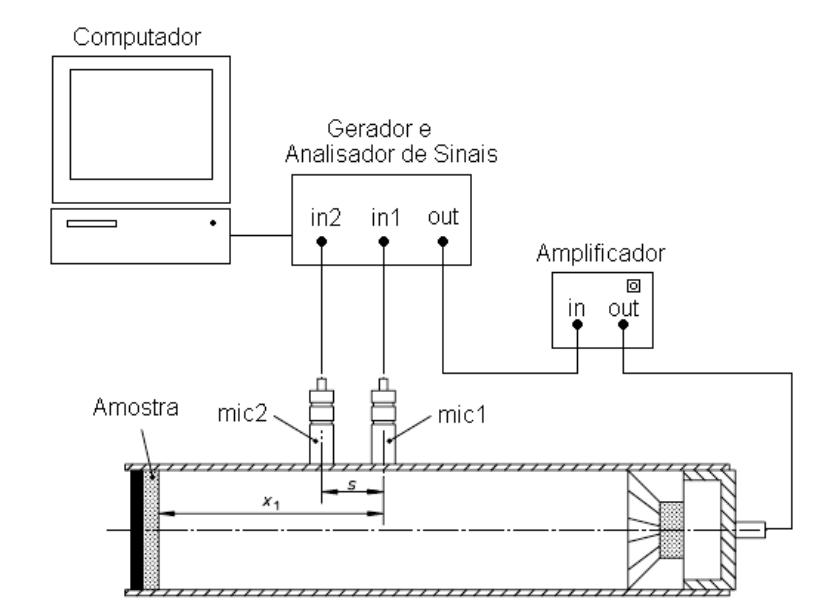
\includegraphics[scale=0.45]{figs/bancada.png}
\caption{Equipamentos utilizados para a medição a determinação do coeficiente de absorção sonora de um material em um tubo de impedância. Fonte \cite{mareze2013analise}}
\label{fig.equipamento}
\end{figure}  

\begin{table}[h]
\centering
\caption{Equipamentos utilizados na medição.}
\label{tab.bancada}
\begin{tabular}{l|l}
Item               & Descrição do Equipamento                                 \\ \hline
1                  & Analisador de sinais B\&K Pulse             \\
2                  & Computador com o programa Pulse LabShop       \\
3                  & Amplificador B\&K 2619\                    \\
4                  & Microfones de 1/2'' modelo B\&K 4189         \\
5                  & Calibrador 200 Larson Davids \\
                                                        
\end{tabular}
\end{table}

O material poroso analisado foi uma lã de vidro produzido pela empresa \textit{Rockfibras}, conforme a Figura \ref{fig.rockfibras}. Primeiramente foi feita a medição da função de transferência entre os microfones sem a presença do material poroso com o intuito de verificar se há absorção sonora nas superfícies do tubo, visto que as superfícies não são idealmente rígidas.
\begin{figure}[h]
\centering
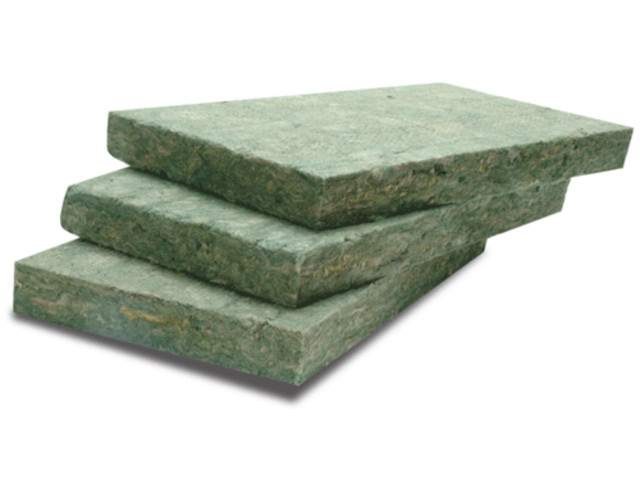
\includegraphics[scale=0.35]{figs/rockfibras.jpg}
\caption{Lã de rocha utilizada para o ensaio.}
\label{fig.rockfibras}
\end{figure}



Posteriormente foi recortada três (3) amostras de lã de vidro do mesmo material, porém com espessuras $h$ ligeiramente diferentes, exibidas na Tabela \ref{tab.espessuras}. O objetivo foi medir separadamente cada uma das amostras e verificar se o coeficiente de absorção sonora teve resultados semelhantes para os três ensaios.

\begin{table}[h]
\centering
\caption{Espessuras das amostras ensaiadas}
\label{tab.espessuras}
\begin{tabular}{l|l}
Item                       & Espessura (mm)      \\ \hline
Amostrador                 & 23.15               \\
Amostra 1                  & 25                  \\
Amostra 2                  & 24.85               \\
Amostra 3                  & 24                  \\
\end{tabular}
\end{table}

Para cada medição foi extraído como resposta as funções de transferências $H_{12}$ através de um \textit{template} programado no software Pulse LabShop. Como já foi discutido anteriormente, a partir das funções de transferência entre os microfones é possível extrair o coeficiente de absorção sonora por incidência direta de um material.

\chapter{Resultados}

%\input{Cap1}

%\input{ConceitosBasicos/ConceitosBasicos}

%\input{Metodos/Metodos}

%\input{Manual/Manual}

%\input{Simulacao/Simulacao}

%\input{Cartas/Cartas}

%\input{Aplicacoes/Aplicacoes}

%\input{Referencias/Referencias}


%%%%%%%%%%%%%%%%%%%%%%%%%%%%%%%%%%%%%%%%%%%%%%%%%%%%%%%%%%%%%%%%%%%%%%%%%%%%%%%%%%
%%%%%%%%%%%%%%%%%%%%%%%%%%%% P s-Textuais
%TC:ignore

%%%%%%%%%%%%%%%% Ref. Bibliograficas
%\cleardoublepage
\phantomsection
%\addcontentsline{toc}{chapter}{Referências Bibliográficas} \label{chap.refs}

% Português
%
\addcontentsline{toc}{part}{References} \label{chap.refs}                   % English

\bibliographystyle{plain}
%\bibliographystyle{abbrv}
%\bibliographystyle{ama}
%\bibliographystyle{unsrt}
\bibliography{Referencias/Referencias.bib} 

%%%%%%%%%%%%%%%% Apendice:
%\cleardoublepage
%\appendix
%\chapter*{Ap ndices}
%\addcontentsline{toc}{chapter}{Ap ndices}
%%\chapter*{Appendix}
%%\addcontentsline{toc}{part}{Appendix}
%
%\mbox{}
%%\input{}

%%%%%%%%%%%%%%%% Anexos:
%\cleardoublepage
%\phantomsection
%\setcounter{chapter}{0}
%\renewcommand{\theHchapter}{an.\Alph{chapter}}
%%\renewcommand{\appendixname}{Anexos} 
%%\addcontentsline{toc}{chapter}{Anexos}
%%\chapter*{Anexos}
%\renewcommand{\appendixname}{Annex} 
%\addcontentsline{toc}{part}{Annex}
%\chapter*{Annex}

%\mbox{}
%\input{}
%%%%%%%%%%%%%%%%%%%
% Pagina em branco
%\blankpage
%%%%%%%%%%%%%%%%%%%%%%%%%%%%%%%%%%%%%%%%%%%%%%%%%%%%%%%%%%%%%%%%%%%%%%%%%%%%%%%%%%
%%%%%%%%%%%%%%%%%%%%%%%%%%%%%%%%%%%%%%%%%%%%%%%%%%%%%%%%%%%%%%%%%%%%%%%%%%%%%%%%%%
\end{document}
%TC:endignore 
%%%%%%%%%%%%%%%%%%%%%%%%%%%%%%%%%%%%%%%%%%%%%%%%%%%%%%%%%%%%%%%%%%%%%%%%%%%%%%%%%%
%%%%%%%%%%%%%%%%%%%%%%%%%%%%%%%%%%%%%%%%%%%%%%%%%%%%%%%%%%%%%%%%%%%%%%%%%%%%%%%%%%